% Phase 1/2 architecture of the word count service (client-server, three tiers).
% Standalone TikZ figure sized for one IEEE column. Compile with
%   pdflatex architecture_phase2.tex
% and include the PDF:  \includegraphics[width=\columnwidth]{figures/architecture_phase2}
% Phase 3 updates this figure with the load balancer and two more server replicas.
\documentclass[tikz,border=1pt]{standalone}
\usepackage{mathptmx}
\usetikzlibrary{positioning,fit,arrows.meta,shapes.geometric,backgrounds,calc}

\begin{document}
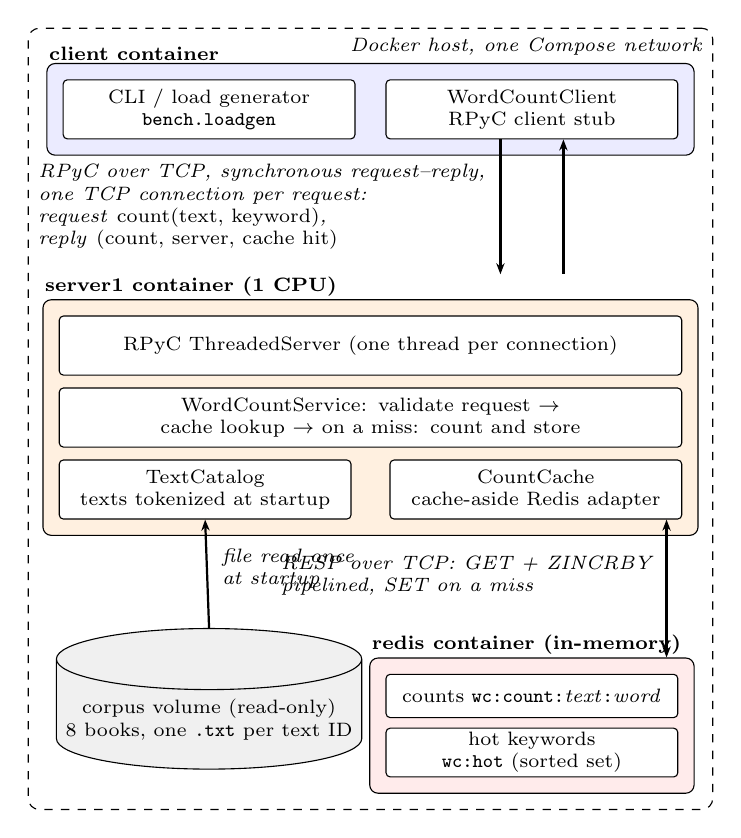
\begin{tikzpicture}[
    >={Stealth[length=4pt,width=3pt]},
    comp/.style={draw, rounded corners=1.5pt, fill=white, align=center, font=\scriptsize,
                 inner sep=1.5pt, minimum height=7.5mm, text width=#1, minimum width=#1},
    comp/.default=36mm,
    box/.style={draw, rounded corners=3pt, inner sep=2mm},
    boxtitle/.style={font=\scriptsize\bfseries, anchor=south west, inner sep=0.8pt},
    lab/.style={font=\scriptsize, align=center, inner sep=1pt},
    note/.style={font=\scriptsize\itshape, align=left, inner sep=1pt},
]
  % ---------------- client tier ----------------
  \node[comp] (cli)  at (2.0, 0) {CLI / load generator\\\texttt{bench.loadgen}};
  \node[comp] (stub) at (6.1, 0) {WordCountClient\\RPyC client stub};
  \begin{scope}[on background layer]
    \node[box, fill=blue!8, fit=(cli)(stub)] (client) {};
  \end{scope}
  \node[boxtitle] (clientT) at (client.north west) {client container};

  % ---------------- application tier ----------------
  \node[comp=78mm] (rpc) at (4.05, -3.0) {RPyC ThreadedServer (one thread per connection)};
  \node[comp=78mm, below=1.5mm of rpc] (svc)
       {WordCountService: validate request $\rightarrow$ cache lookup $\rightarrow$ on a miss: count and store};
  \node[comp, below=1.5mm of svc.south west, anchor=north west] (cat) {TextCatalog\\texts tokenized at startup};
  \node[comp, below=1.5mm of svc.south east, anchor=north east] (cache) {CountCache\\cache-aside Redis adapter};
  \begin{scope}[on background layer]
    \node[box, fill=orange!12, fit=(rpc)(svc)(cat)(cache)] (server) {};
  \end{scope}
  \node[boxtitle] (serverT) at (server.north west) {server1 container (1 CPU)};

  % ---------------- data tier ----------------
  \node[comp, minimum height=5.5mm] (counts) at (6.1, -7.45) {counts \texttt{wc:count:}\textit{text}\texttt{:}\textit{word}};
  \node[comp, minimum height=5.5mm, below=1.2mm of counts] (hot) {hot keywords \texttt{wc:hot} (sorted set)};
  \begin{scope}[on background layer]
    \node[box, fill=red!8, fit=(counts)(hot)] (redis) {};
  \end{scope}
  \node[boxtitle] (redisT) at (redis.north west) {redis container (in-memory)};
  \node[draw, cylinder, shape border rotate=90, aspect=0.2, fill=gray!12, align=center, font=\scriptsize,
        minimum width=36mm, minimum height=12mm] (corpus) at (2.0, -7.75)
        {corpus volume (read-only)\\8 books, one \texttt{.txt} per text ID};

  % ---------------- connectors ----------------
  % client -> server: RPyC
  \coordinate (reqTop) at ([xshift=-4mm]stub.south);
  \coordinate (repTop) at ([xshift=4mm]stub.south);
  \draw[->, thick] (reqTop) -- (reqTop |- serverT.north);
  \draw[<-, thick] (repTop) -- (repTop |- serverT.north);
  \node[note, anchor=east] at ($(reqTop)!0.5!(reqTop |- serverT.north) + (-1.5mm, 0)$)
       {RPyC over TCP, synchronous request--reply,\\one TCP connection per request:\\request \textup{count(text, keyword)},\\reply \textup{(count, server, cache hit)}};
  % server -> redis: RESP
  \coordinate (respTop) at ([xshift=-2mm]cache.south east);
  \draw[<->, thick] (respTop) -- (respTop |- redis.north);
  \node[note, anchor=east] at ($(respTop)!0.5!(respTop |- redisT.north) + (-1.5mm, 0)$)
       {RESP over TCP: GET + ZINCRBY\\pipelined, SET on a miss};
  % corpus -> server: file read
  \draw[->, thick] (corpus.north) -- (cat.south);
  \node[note, anchor=west] at ($(corpus.north)!0.55!(cat.south) + (1.5mm, 0)$) {file read once\\at startup};

  % ---------------- deployment boundary ----------------
  \begin{scope}[on background layer]
    \node[draw, dashed, rounded corners=4pt, inner xsep=1.8mm, inner ysep=2mm,
          fit=(clientT)(client)(server)(redis)(corpus)] (host) {};
  \end{scope}
  \node[font=\scriptsize\itshape, anchor=north east, inner sep=1.2pt] at ([xshift=-1mm, yshift=-0.8mm]host.north east)
       {Docker host, one Compose network};
\end{tikzpicture}
\end{document}
